\documentclass{article}
\usepackage{import}
\usepackage{graphicx}
\usepackage[utf8]{inputenc}
\usepackage[section]{placeins}
\usepackage[english]{babel}
\usepackage{amsmath}
\usepackage{csquotes}
\usepackage{biblatex}
\bibliography{ref.bib}

\title{ETERNITY: NUMBERS - Silver Ratio $(\delta_s)$}
\author{Md Hasibul Huq}
\date{July 2019}

\begin{document}               % plus the \end{document} command at the end.
\maketitle

\section{Introduction}          % This command makes a section title.

This document provides an understanding of only an irrational  number called Silver Ratio $(\delta_s)$. An irrational  number is  not  a rational  number, it is not possible to express an irrational number as a quotient of two integers \cite{project_des}.
\subsection{History}
Silver Ratio is studied from the time of Greek knowledge, which discusses the fundamental characteristics of the number system. Though it is not used by normal people intentionally. Silver ratio is the limiting of consecutive  of infinite sequence of integers, The silver ratio is presented in a Greek symbol ($\delta_s$).

\subsection{Mathematical Definition}
The value of silver ration is 2.4142135623 \cite{jdc_silver}. A ratio of the sequential sum of smaller number and twice of the larger number, which will produce an infinite sequence and the ration between smaller and larger number will be always same \cite{numberphile_silver}. This can be presented in mathematical equation:- 

\[ \dfrac{2a + b}{a}  = \dfrac{b}{a} = \delta_s \]

It will be easier to understand if it can be compared with Fibonacci number.
In Fibonacci, the smaller and larger number are added to get the next one. 
Example:-

$$1,1,2,3,5,8,13,..$$

For silver ratio, the smaller and twice of the larger number are added to get the next one. Example:-

\[1,2,5,12,29,70,..\] 

Then the latest number is divided  by the previous larger number. 

\section{Interview}
I interviewed a undergraduate student from Dhaka University - Bangladesh with math background. Her name is Esrat Jahan Tonni. As she is currently studying, she might need to use irrational numbers in her undergraduate career. The interview questions and the answers are given below:-\newline

\subsection{Question and Answer}
Q1: How long you are in math domain? \newline
Ans: Almost 3 years.\newline\newline
Q2: How often you use calculator?\newline
Ans: Very often. I mean almost daily.\newline \newline
Q3:What type of device you use to calculate complex equation.\newline
Ans:It is obviously scientific calculator for me but for advance user there are many software available.\newline\newline
Q4: Can you tell me some of the tools name?\newline
Ans: No. I can't remember the names but if you search it in Google you will find some.\newline\newline
Q5: Do you know about the irrational number?\newline
Ans: Yes. I Know,\newline\newline
Q6: Do you know about Silver Ratio?\newline
Ans: I am not sure. I think, I know about it but never used it . But have some basic idea about it. \newline\newline
Q7: Can you explain me what you know about it?\newline
Ans: I am not sure. But so far I can remember i will try to give you a basic idea of it. Hopefully you heard the name of Fibonacci number. It is related to Golden Ratio. Same as there is Silver ratio. It has some difference with golden ratio.It actually describe the twice  of the larger number added with the previous number and ratio with previous number.\newline\newline
Q8: Do you know the value of silver ratio?\newline
Ans: It is something one plus square root of two. I forget the value. It will be something 2.414 and more \newline\newline
Q9:What do you think are the applications of the Golden Ratio in mathematics?\newline
Ans: The silver ratio is used mostly in the Geometry to create designs that are in proportions. It is not used as such in Mathematics directly but even the ratio of consecutive numbers in Pell sequence are close to the silver ratio. \newline\newline
Q10: What are the other places where it can help?\newline
Ans: It is usually used in the geometrical calculation.As well as the architect and engineers uses this to make shapes calculation.It may be used in art and design, some time it helps in surgery to measure some points.  \newline\newline
Q11: Can you give me some example where it can be implemented\newline
Ans: To make a perfect square it helps. Octagon is another example where you need this.\newline\newline
Q12: Do your scientific calculator support silver ratio?\newline
Ans: Never used that. so I am not sure about it. it may be or may not be.\newline\newline
Q13: Would you like to include Irrational constants like silver ratio and others in the calculator? \newline
Ans: Yes. Why not may be in future i need them.\newline\newline
Q14: Do you have any other suggestion that can help me to find your necessity in a scientific calculator?\newline
Ans: Currently, I don't need any other feature in my calculator. but who knows if can come up with something new it may help others.\newline\newline

\subsection{Interview  Analysis}
Though the interviewee is not expert in the area of the irrational numbers, She has decent idea about the silver ratio. As she has a math background, she gave a lots of insights about the silver ratio. She is 4th Year student and completed 3 years in math domain. As a math student she has to use calculator almost everyday and she uses scientific calculator for the complex equations. From the interview, it is clear that the silver ratio is used in calculation of geometrical shapes. Also the architect, designer, engineers and Sometimes doctors (Plastic Surgery) uses this. Also stated that in regular scientific calculator the irrational numbers are not available. Then she describe about the silver ratio . which has the value of 4142135623.Its convergent are square triangular numbers, Pell numbers and octagons. According to her it will be good if the irrational numbers are included in the scientific calculator. According to him the calculation can be done here in the scientific calculators but they needs extra effort. But inclusion of these can make few peoples life easier. 

\section{Persona}
The persona is given below: 
\begin{figure}[htb!]
  
  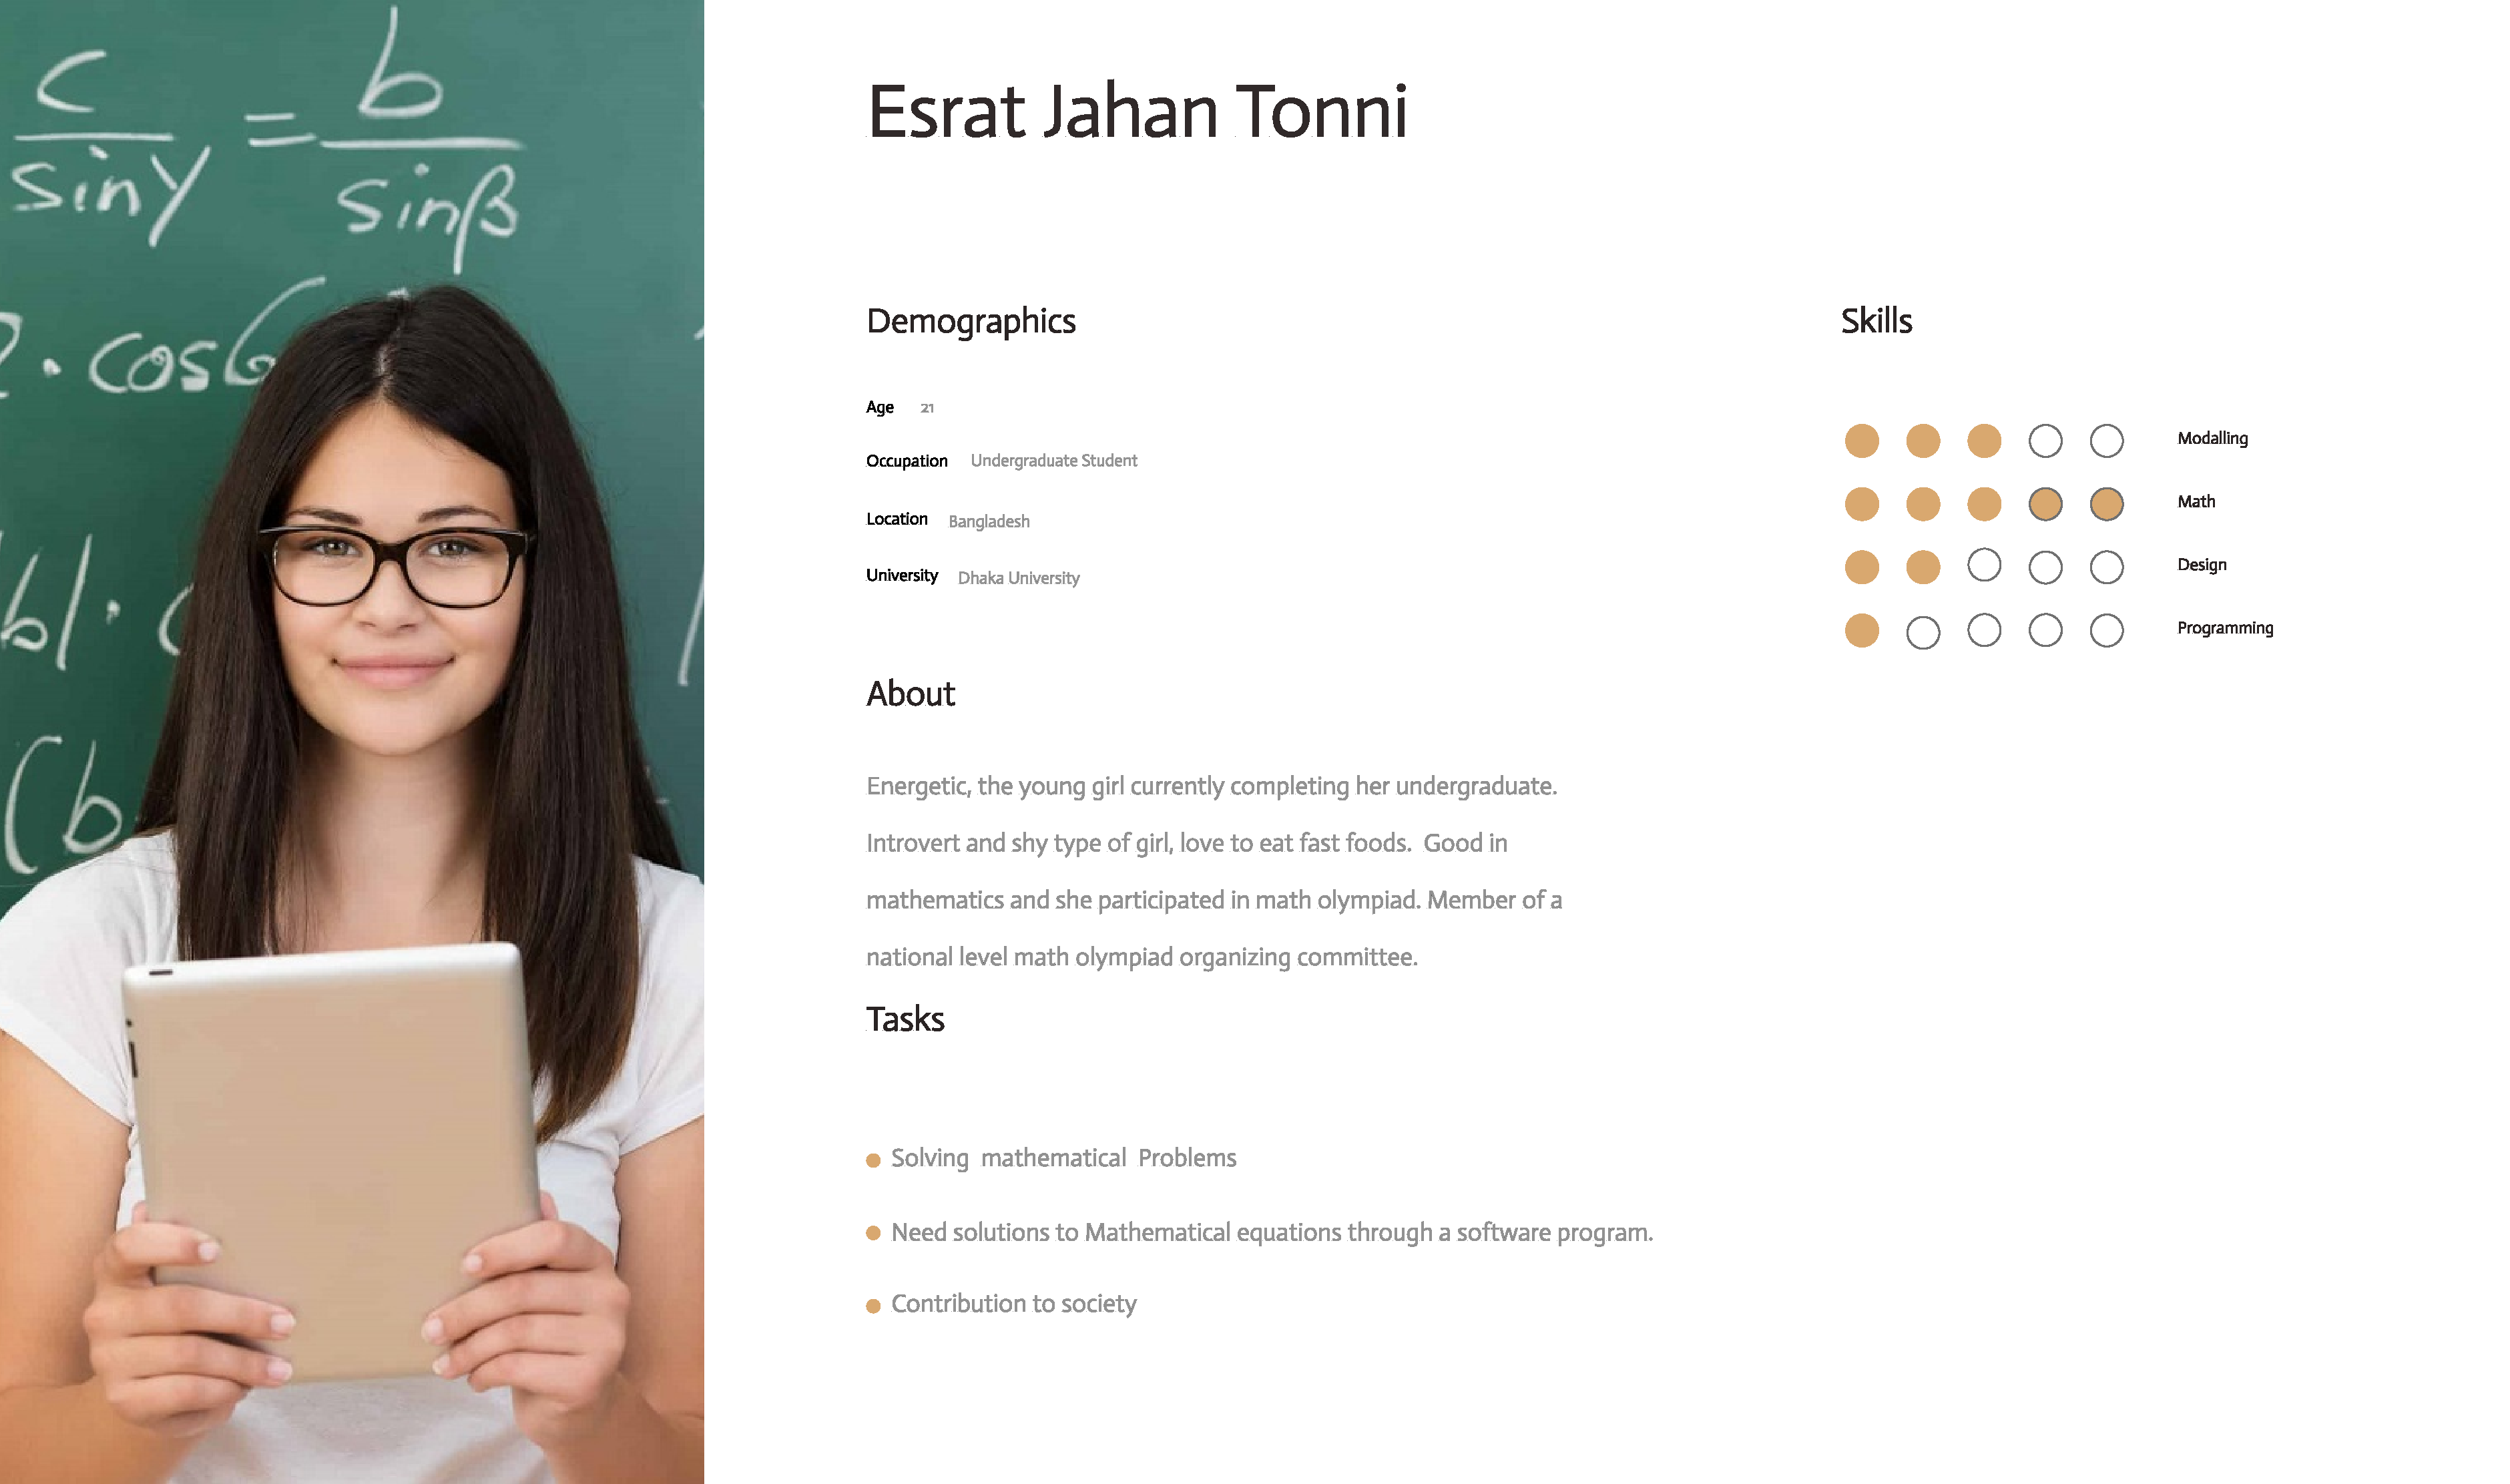
\includegraphics[width=1\textwidth]{persona}
  \centering
  \caption{Persona based on the analysis of interview}
\end{figure}

\section{Problem Domain Model}
\begin{figure}[htb!]
  
  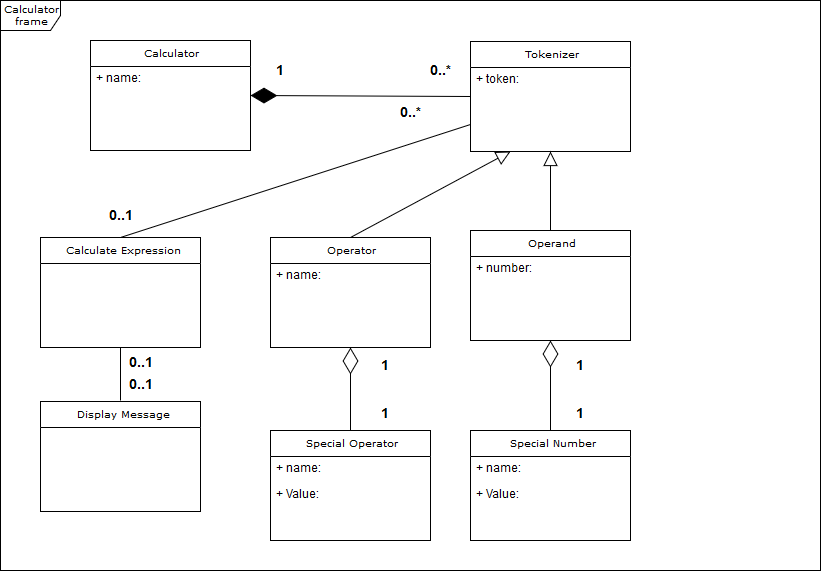
\includegraphics[width=1\textwidth]{uml}
  \centering
  \caption{Class diagram for calculator with special number and operator}
\end{figure}

\section{Use case Model}

\subsection{Use Case Diagram}
Actor of this system will be an user. The user will give inputs of operator and operands. User can sometimes use special operator. but it is optional to use. Same for the operand input field can have any number. but if the user wants can have special number like Silver Ratio. With the Operator and operand it makes an mathematical expression. Calculate the expression and display the result. 
\begin{figure}[htb!]
  
  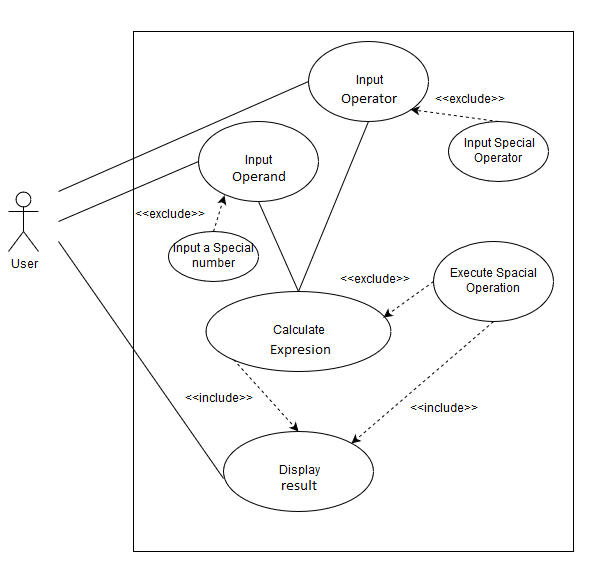
\includegraphics[width=1\textwidth]{usecase}
  \centering
  \caption{Use case diagram for calculator with special number and operator}
\end{figure}
\subsection{Activity Diagram}
Here it will work like a regular calculator with an extra feature of an operand silver ratio number and operator for getting a value from a number using the silver ratio content.
If silver ratio is used as a operand it will work like a double number.
An example is given below :- 
$$2+\delta_s = 4.4142$$
\begin{figure}[!htb]
 \centering
  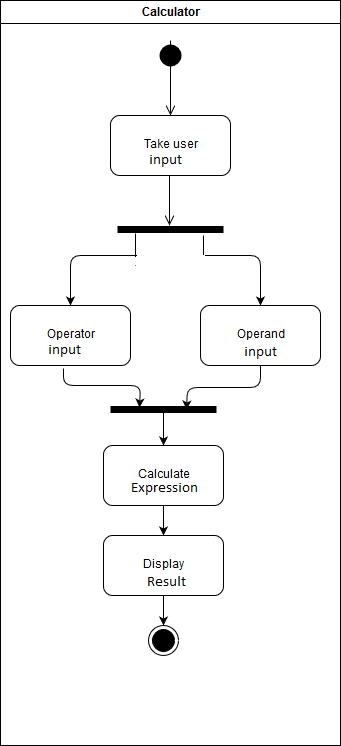
\includegraphics[width=.50\textwidth]{activity}
  \caption{Activity diagram for calculator with special number and operator}
\end{figure}

if it uses like an operator than it will give the value of the another number which ratio is $\delta_s$. If one value is 2 than the silver ratio operand will give the another value (0.82842712474619 )based on the silver ratio equation.
the equation is give below: - \newline

\[ \dfrac{2a + b}{a}  = \delta_s \]
\[ => {2a + b}  = {a *\delta_s} \]
\[ => {b}  = {(a *\delta_s) - 2a} \]

\section{User Stories}
\subsection{Global Constraints}
\begin{itemize}
  \item The information about silver ratio is available in the internet. But the application of this ratio is not clear. This irrational number is used in many geometrical calculation but the use of that is not available in internet. 
  \item Geometric interpretation of the silver ratio is not clearly mentioned \cite{jdc_silver}.
\end{itemize}

\subsection{Local Constraints}
Interviewee doesn't apply silver ratio in his career. So he exactly doesn't know how it helps. But he has a conceptual idea about the ratio. 

\subsection{User Stories (US)}
The concept of the type of user stories are taken from online search\cite{js_story,cal_story}. And the user story presented here are based on interview and use case model from this document. \newline

\begin{tabular}{ |p{2cm}|p{5cm}|p{2cm}|p{4cm}| }
 \hline
 \multicolumn{4}{|c|}{US 1 - Input the digital numbers} \\
 \hline
 \textbf {Story ID}& US1 &  \textbf{Priority} & HIGH \\
 \hline
  \textbf{Description}   & As an user, I want click able 0 to 9 numbers in calculator &    \textbf{Acceptance Test}& 
\begin{itemize}
\item Click 2 twice and click on any operator number. it will save 22 in a variable.
\end{itemize}
  \\
 \hline
 \textbf{Estimate} & 0.5 d &  \textbf{Constrains}& Number has to be in this range $9999999999>x>-9999999999$  \\
 \hline
 \textbf{Acceptance Criteria} & When i click them they will store it in a variable until i click any operator or a equal sign.  &  \textbf{Implement- ed}& Yes  \\
 \hline
\end{tabular}

\begin{tabular}{ |p{2cm}|p{5cm}|p{2cm}|p{4cm}| }
 \hline
 \multicolumn{4}{|c|}{US 2 - Addition of two numbers} \\
 \hline
 \textbf {Story ID}& US2 &  \textbf{Priority} & HIGH \\
 \hline
  \textbf{Description}   & As an user, I want add two numbers so that I can see what is the total number &    \textbf{Acceptance Test}& 
\begin{itemize}
\item Given two numbers need to be added and have to return the total result. Example: 14 add 7 will produce the result 21. 6 add 4 will produce the result 10. 
\end{itemize}
  \\
 \hline
 \textbf{Estimate} & 0.2 d &  \textbf{Constrains}&   Addition with a minus number can work like a subtraction.\\
 \hline
 \textbf{Acceptance Criteria} & 
 \begin{itemize}
\item Click on 1 button
\item Click on 4 button
\item Click on + button
\item Click on 7 button
\item Click on = button
\item It will give you 21 as a result 
\end{itemize}
 &  \textbf{Implement- ed}& Yes  \\
 \hline
\end{tabular}

\begin{tabular}{ |p{2cm}|p{5cm}|p{2cm}|p{4cm}| }
 \hline
 \multicolumn{4}{|c|}{US 3 - Subtraction of two numbers} \\
 \hline
 \textbf {Story ID}& US3 &  \textbf{Priority} & HIGH \\
 \hline
  \textbf{Description}   & As an user, I want subtract two numbers so that I can see what is the result &    \textbf{Acceptance Test}& 
\begin{itemize}
\item Given two numbers need to be subtracted and have to return the rest. Example: 7 subtracted from 14 will produce the result 7. 6 subtracted from 10 will produce the result 4. 
\end{itemize}
  \\
 \hline
 \textbf{Estimate} & 0.1 d &  \textbf{Constrains}&  If the number which will be subtracted is bigger than actual number it will produce minus result  \\
 \hline
 \textbf{Acceptance Criteria} & 
 \begin{itemize}
\item Click on 1 button
\item Click on 4 button
\item Click on - button
\item Click on 7 button
\item Click on = button
\item It will give you 7 as a result 
\end{itemize}
 &  \textbf{Implement- ed}& Yes  \\
 \hline
\end{tabular}

\begin{tabular}{ |p{2cm}|p{5cm}|p{2cm}|p{4cm}| }
 \hline
 \multicolumn{4}{|c|}{US 4 - Multiplication of two numbers} \\
 \hline
 \textbf {Story ID}& US4 &  \textbf{Priority} & HIGH \\
 \hline
  \textbf{Description}   & As an user, I want multiply two numbers so that I can see what is the result &    \textbf{Acceptance Test}& 
\begin{itemize}
\item Given two numbers need to be multiplied and have to return the result. Example: 14 multiplied with 7 will produce the result 98. 6 multiplied with 10 will produce the result 60. 
\end{itemize}
  \\
 \hline
 \textbf{Estimate} & 0.1 d &  \textbf{Constrains}&  If the number which will be multiplied is less than zero it will produce a minus number and  less than 1 but greater than zero will reduce the number. \\
 \hline
 \textbf{Acceptance Criteria} & 
 \begin{itemize}
\item Click on 1 button
\item Click on 4 button
\item Click on * button
\item Click on 7 button
\item Click on = button
\item It will give you 98 as a result 
\end{itemize}
 &  \textbf{Implement- ed}& Yes  \\
 \hline
\end{tabular}

\begin{tabular}{ |p{2cm}|p{5cm}|p{2cm}|p{4cm}| }
 \hline
 \multicolumn{4}{|c|}{US 5 - Division of two numbers} \\
 \hline
 \textbf {Story ID}& US5 &  \textbf{Priority} & HIGH \\
 \hline
  \textbf{Description}   & As an user, I want divide two numbers so that I can see what is the division result &    \textbf{Acceptance Test}& 
\begin{itemize}
\item Given two numbers need to be divided and have to return the result. Example: 14 divided by 7 will produce the result 2. 16 divided by 2 will produce the result 8. 
\end{itemize}
  \\
 \hline
 \textbf{Estimate} & 0.1 d &  \textbf{Constrains}&  No number can be divided by zero. \\
 \hline
 \textbf{Acceptance Criteria} & 
 \begin{itemize}
\item Click on 1 button
\item Click on 4 button
\item Click on / button
\item Click on 7 button
\item Click on = button
\item It will give you 2 as a result 
\end{itemize}
 &  \textbf{Implement- ed}& Yes  \\
 \hline
\end{tabular}

\begin{tabular}{ |p{2cm}|p{5cm}|p{2cm}|p{4cm}| }
 \hline
 \multicolumn{4}{|c|}{US 6 - Toggle a number} \\
 \hline
 \textbf {Story ID}& US6 &  \textbf{Priority} & Low \\
 \hline
  \textbf{Description}   & As an user, I want toggle the sign of the number so that i can get opposite value &    \textbf{Acceptance Test}& 
\begin{itemize}
\item Given number need to be opposite sign number. Example: 4 will be -4.   -6 will be 6. 
\end{itemize}
  \\
 \hline
 \textbf{Estimate} & 0.1 d &  \textbf{Constrains}&   \\
 \hline
 \textbf{Acceptance Criteria} & 
 \begin{itemize}
\item Click on 4 button
\item Click on +/- button
\item It will give you -4 as a result 
\end{itemize}
 &  \textbf{Implement- ed}& Yes  \\
 \hline
\end{tabular}

\begin{tabular}{ |p{2cm}|p{5cm}|p{2cm}|p{4cm}| }
 \hline
 \multicolumn{4}{|c|}{US 7 - Equal operation} \\
 \hline
 \textbf {Story ID}& US7 &  \textbf{Priority} & High \\
 \hline
  \textbf{Description}   & As an user, I want every calculation result after clicking in the equal button &    \textbf{Acceptance Test}& 
\begin{itemize}
\item For US2 to US5 all the use case result will be displayed if the user press equal button. 
\end{itemize}
  \\
 \hline
 \textbf{Estimate} & 0.1 d &  \textbf{Constrains}& If there is no operation occurred it will show the current value in display   \\
 \hline
 \textbf{Acceptance Criteria} & 
 \begin{itemize}
\item Click on 1 button
\item Click on 4 button
\item Click on + button
\item Click on 7 button
\item Click on = button
\item It will give you 21 as a result 
\end{itemize}
 &  \textbf{Implement- ed}& Yes  \\
 \hline
\end{tabular}

\begin{tabular}{ |p{2cm}|p{5cm}|p{2cm}|p{4cm}| }
 \hline
 \multicolumn{4}{|c|}{US 8 - Silver ratio as a operand} \\
 \hline
 \textbf {Story ID}& US8 &  \textbf{Priority} & High \\
 \hline
  \textbf{Description}   & As an user, I want the button of silver ratio as number. So that i can use it as a number for arithmetic operation. &    \textbf{Acceptance Test}& 
\begin{itemize}
\item  If you click the button it will be equivalent to 2.4142135623. So all the arithmetic operation will occur with this operand. Example : 5 + $(\delta_s)$ = 7.4142135623, $(\delta_s)$ - 1.4142135623 = 1
\end{itemize}
  \\
 \hline
 \textbf{Estimate} & 0.1 d &  \textbf{Constrains}&  can not be divided by zero.  \\
 \hline
 \textbf{Acceptance Criteria} & 
 \begin{itemize}
\item Click on $(\delta_s)$ button
\item It will give you 2.4142135623 as a value 
\end{itemize}
 &  \textbf{Implement- ed}& Yes  \\
 \hline
\end{tabular}

\begin{tabular}{ |p{2cm}|p{5cm}|p{2cm}|p{4cm}| }
 \hline
 \multicolumn{4}{|c|}{US 9 - Silver ratio as a operator} \\
 \hline
 \textbf {Story ID}& US9 &  \textbf{Priority} & High \\
 \hline
  \textbf{Description}   & As an user, I want to know the number for which silver ratio will be a given number. &    \textbf{Acceptance Test}& 
\begin{itemize}
\item  The silver ratio of 2 will be 0.82842712474619.
\end{itemize}
  \\
 \hline
 \textbf{Estimate} & 0.1 d &  \textbf{Constrains}&  The ratio of zero is not possible.  \\
 \hline
 \textbf{Acceptance Criteria} & 
 \begin{itemize}
\item Click on 2 button
\item Click on $(\delta_s)$ -op button
\item It will give you 0.82842712474619. as a result 
\end{itemize}
 &  \textbf{Implement- ed}& Yes  \\
 \hline
\end{tabular}

\begin{tabular}{ |p{2cm}|p{5cm}|p{2cm}|p{4cm}| }
 \hline
 \multicolumn{4}{|c|}{US 10 -  Decimal separator} \\
 \hline
 \textbf {Story ID}& US10 &  \textbf{Priority} & High \\
 \hline
  \textbf{Description}   & As an user, I want to use decimal number so I want a decimal separator for decimal number input. &    \textbf{Acceptance Test}& 
\begin{itemize}
\item  Need to take decimal input.
\end{itemize}
  \\
 \hline
 \textbf{Estimate} & 0.1 d &  \textbf{Constrains}&  Decimal separator can be used once in a number.  \\
 \hline
 \textbf{Acceptance Criteria} & 
 \begin{itemize}
\item Click on 2 button
\item Click on .  button
\item Click on 2 button
\item It will give you 2.2 as a value 
\end{itemize}
 &  \textbf{Implement- ed}& Yes  \\
 \hline
\end{tabular}

\begin{tabular}{ |p{2cm}|p{5cm}|p{2cm}|p{4cm}| }
 \hline
 \multicolumn{4}{|c|}{US 11 -  Square} \\
 \hline
 \textbf {Story ID}& US11 &  \textbf{Priority} & Medium \\
 \hline
  \textbf{Description}   & As an user, I want to use the square value of a given number. &    \textbf{Acceptance Test}& 
\begin{itemize}
\item  The value will be the multiplication of it's own. 2 square is 4
\end{itemize}
  \\
 \hline
 \textbf{Estimate} & 0.1 d &  \textbf{Constrains}&  For Square of non positive number, the sign of the number will be changed. For -2 it will be 4.  \\
\hline
 \textbf{Acceptance Criteria} & 
 \begin{itemize}
\item Click on 2 button
\item Click on x*x button
\item It will give you 4. as a result 
\end{itemize}
 &  \textbf{Implement- ed}& Yes  \\
 \hline
\end{tabular}

\begin{tabular}{ |p{2cm}|p{5cm}|p{2cm}|p{4cm}| }
 \hline
 \multicolumn{4}{|c|}{US 12 -  Square Root} \\
 \hline
 \textbf {Story ID}& US12 &  \textbf{Priority} & Medium \\
 \hline
  \textbf{Description}   & As an user, I want to use the square root value of a given number. &    \textbf{Acceptance Test}& 
\begin{itemize}
\item  The value will be the a number which square is the given number. 4 square root is 2.  
\end{itemize}
  \\
 \hline
 \textbf{Estimate} & 0.1 d &  \textbf{Constrains}&    \\
 \hline
 \textbf{Acceptance Criteria} & 
 \begin{itemize}
\item Click on 4 button
\item Click on root button
\item It will give you 2. as a result 
\end{itemize}
 &  \textbf{Implement- ed}& Yes  \\
 \hline
\end{tabular}

\section{Traceability Matrix}

The traceability matrix is realized to ensure that all the requirements defined for the system are tested and passed \cite{prev_project}.\newline

\begin{tabular}{ |p{1cm}|p{1cm}|p{1cm}|p{3cm}|p{3cm}|p{2cm}| }
\hline
 ID & REQ ID & REQ TYPE & REQ DESC & REQ SRC  & FLAG \\
 \hline
  US1 & 1 & FN & As an user, I want click able 0 to
9 numbers in calculator & System description from Deliverable 1 (D1) and ref \cite{js_story} & Passed \\
 \hline
 US2 & 2 & FN & As an user, I want add two numbers so that I can see what is the
total number & Class diagram from D1. as operator & Passed \\
 \hline
 US3 & 3 & FN & As an user, I want subtract two
numbers so that I can see what
is the result & Class diagram from D1. as operator  & Passed \\
 \hline
 US4 & 4 & FN & As an user, I want multiply two
numbers so that I can see what
is the result & Class diagram from D1. as operator  & Passed \\
 \hline
\end{tabular}


\begin{tabular}{ |p{1cm}|p{1cm}|p{1cm}|p{3cm}|p{3cm}|p{2cm}| }
 \hline
  US5 & 5 & FN & As  an  user,  I  want  divide  two
numbers so that I can see what
is the division result & Class diagram from D1. as operator  & Passed \\
 \hline
 US6 & 6 & FN & As an user, I want toggle the sign
of the number so that i can get
opposite value & System description from Deliverable 1 (D1) and ref \cite{cal_story}  & Passed \\
 \hline
 US7 & 7 & FN & As  an  user,  I  want  every  calculation result after clicking in the
equal button & REQ ID 2,3,4,5  & Passed \\
 \hline
 US8 & 8 & FN & As an user, I want the button of
silver ratio as number.  So that i
can use it as a number for arithmetic operation. & Use case diagram from D1  & Passed \\
 \hline
 US9 & 9 & FN & As an  user,  I want  to know the
number for which silver ratio will
be a given number. & Use case diagram from D1  & Passed \\
 \hline
 US10 & 10 & FN & As an user, I want to use decimal
number so I want a decimal separator for decimal number input & System description from Deliverable 1 (D1) and ref \cite{js_story}  & Passed \\
\hline
 US11 & 11 & FN & As  an  user,  I  want  to  use  the
square value of a given number. The value will be the
multiplication of it’s own.  2 square is 4 & Use case from D1  & Passed \\
 \hline
 US12 & 12 & FN & As  an  user,  I  want  to  use  the
square root value of a given number. & Use case from D1 & Passed \\
\hline
\end{tabular}

\section{Implementation}
Based on a set of user stories a calculator is build by java programming language. The calculator is having basic calculator operation as well as  it has some special operation based on the user stories and use cases. Some operation based on silver ratio is in the calculation. All the user stories are implemented in this project. The logical concept is taken from another project \cite{cal_project}.
\begin{figure}[!htb]
 \centering
  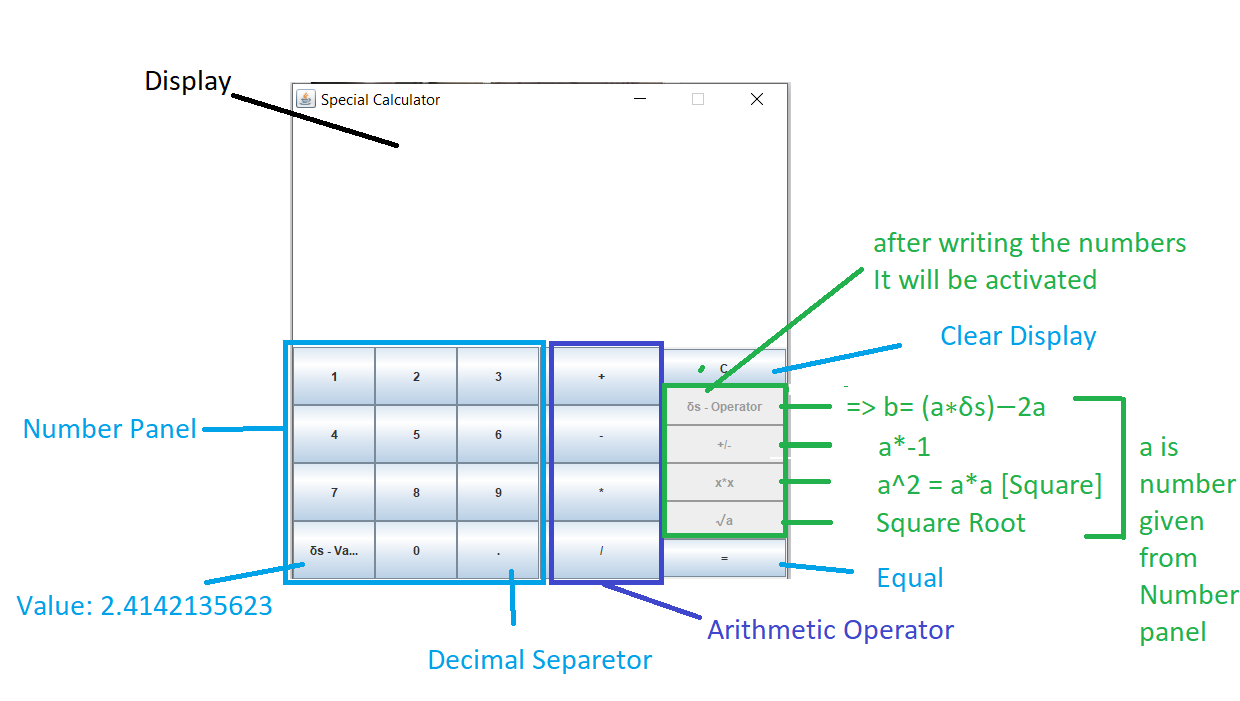
\includegraphics[width=1\textwidth]{project}
  \caption{Screen Shot of the implemented calculator.}
\end{figure}

The project itself contains the java files along with jar file of this application. The JUnit test case file is also added with the java file named "CalculatorTest.java". The project link is also given in the online version section in this report along with the link of digital copy of this report. 
\section{Online Version}
\textbf{Report:} \url{https://github.com/Hasib-rafi1/SRS-Silver-Ratio}
\newline
\textbf{Project:} \url{https://github.com/Hasib-rafi1/srs-project-calculator}\newline

\section{Conclusion}
In this document, the user stories for the calculator system have been written to capture basic requirement of a calculator system along with silver ratio. This user stories are implemented by java program where all the acceptance test are passed. This document contains both the D1 and D2. 
\printbibliography
\end{document}                 % The input file ends with this command.
